\documentclass{instrukcja}
\usepackage[polish]{babel}
\usepackage[utf8]{inputenc}
\usepackage[OT4]{fontenc}

\begin{document}

\materialnumber{2}
\course[MetNum]{Metody Numeryczne}
\material[Lab 2]{Instrukcja 2}
\author{B. Górecki}
\materialtitle

\section*{Wprowadzenie}

Niniejszą instrukcją rozpoczynamy cykl laboratoriów, z których każde kolejne będzie rozwinięciem poprzedniego i wnioski z poprzedniego będą stanowiły motywację do zastosowania kolejnych metod. Tym samym należy zadbać o to, aby zadania z każdego laboratorium były wykonywane do końca, czy to na zajęciach czy w domu. Dziś zaznajomimy się ze sformułowaniem metody elementów skończonych dla jednego elementu czworokątnego. Dla uproszczenia nie będziemy stosować transformacji geometrycznych występujących w rzeczywistym sformułowaniu metody elementów skończonych, więc faktycznie będziemy operować zawsze na jednostkowych elementach kwadratowych.

\section{Sformułowanie algebraiczne dla jednego elementu}
Zagadnienie wytrzymałości konstrukcji dla jednego elementu skończonego ma następujące sformułowanie algebraiczne: Elementowi skończonemu przypisana jest tzw. macierz sztywności $K$ reprezentująca jego sztywność na poszczególne rodzaje odkształceń (przesunięć jego wierzchołków), wektor przesunięć $\vec d$, jakim ulegną poszczególne wierzchołki elementu pod obciążeniem oraz wektor sił węzłowych $\vec F$ reprezentujący odpowiednio przeliczone siły (bądź obciążenia ciągłe) przyłożone do węzłów elementu.

\begin{displaymath}
K \vec d = \vec F
\end{displaymath}

Wektor przesunięć (ang. {\it displacement}) zawiera odpowiednio przesunięcia względem osi $x$ oraz $y$ kolejnych węzłów elementu (numeracja węzłów pokazana jest na Rysunku 1). Wektor sił węzłowych $\vec F$ ma analogiczną postać. Poniżej przedstawiona jest również macierz sztywności $K$.

\begin{displaymath}
\vec d = \left[ \begin{tabular}{c} $x_0$ \\ $y_0$ \\ $x_1$ \\ $y_1$ \\ $x_2$ \\ $y_2$ \\ $x_3$ \\ $y_3$ \\ \end{tabular} \right] \quad \quad \quad \vec F = \left[ \begin{tabular}{c} $F_{x_0}$ \\ $F_{y_0}$ \\ $F_{x_1}$ \\ $F_{y_1}$ \\ $F_{x_2}$ \\ $F_{y_2}$ \\ $F_{x_3}$ \\ $F_{y_3}$ \\ \end{tabular} \right]
\end{displaymath}
\begin{displaymath}
 K = \frac{E}{1-\nu^2} \left[ \begin{tabular}{c c c c c c c c} $\frac{1}{2} - \frac{\nu}{6}$ & $\frac{1}{8} + \frac{\nu}{8}$ & $-\frac{1}{4} - \frac{\nu}{12}$ & $-\frac{1}{8} + \frac{3}{8}\nu$ & $-\frac{1}{4} + \frac{\nu}{12}$ & $-\frac{1}{8} - \frac{\nu}{8}$ & $\frac{\nu}{6}$ & $\frac{1}{8} - \frac{3}{8}\nu$ \\
$\frac{1}{8} + \frac{\nu}{8}$ & $\frac{1}{2} - \frac{\nu}{6}$ & $\frac{1}{8} - \frac{3}{8}\nu$ & $\frac{\nu}{6}$ & $-\frac{1}{8} - \frac{\nu}{8}$ & $-\frac{1}{4} + \frac{\nu}{12}$ & $-\frac{1}{8} + \frac{3}{8}\nu$ & $-\frac{1}{4} - \frac{\nu}{12}$ \\
$-\frac{1}{4} - \frac{\nu}{12}$ & $\frac{1}{8} - \frac{3}{8}\nu$ & $\frac{1}{2} - \frac{\nu}{6}$ & $-\frac{1}{8} - \frac{\nu}{8}$ & $\frac{\nu}{6}$ & $-\frac{1}{8} + \frac{3}{8}\nu$ & $-\frac{1}{4} + \frac{\nu}{12}$ & $\frac{1}{8} + \frac{\nu}{8}$ \\
$-\frac{1}{8} + \frac{3}{8}\nu$ & $\frac{\nu}{6}$ & $-\frac{1}{8} - \frac{\nu}{8}$ & $\frac{1}{2} - \frac{\nu}{6}$ & $\frac{1}{8} - \frac{3}{8}\nu$ & $-\frac{1}{4} - \frac{\nu}{12}$ & $\frac{1}{8} + \frac{\nu}{8}$ & $-\frac{1}{4} + \frac{\nu}{12}$ \\
$-\frac{1}{4} + \frac{\nu}{12}$ & $-\frac{1}{8} - \frac{\nu}{8}$ & $\frac{\nu}{6}$ & $\frac{1}{8} - \frac{3}{8}\nu$ & $\frac{1}{2} - \frac{\nu}{6}$ & $\frac{1}{8} + \frac{\nu}{8}$ & $-\frac{1}{4} - \frac{\nu}{12}$ & $-\frac{1}{8} + \frac{3}{8}\nu$ \\
$-\frac{1}{8} - \frac{\nu}{8}$ & $-\frac{1}{4} + \frac{\nu}{12}$ & $-\frac{1}{8} + \frac{3}{8}\nu$ & $-\frac{1}{4} - \frac{\nu}{12}$ & $\frac{1}{8} + \frac{\nu}{8}$ & $\frac{1}{2} - \frac{\nu}{6}$ & $\frac{1}{8} - \frac{3}{8}\nu$ & $\frac{\nu}{6}$ \\
$\frac{\nu}{6}$ & $-\frac{1}{8} + \frac{3}{8}\nu$ & $-\frac{1}{4} + \frac{\nu}{12}$ & $\frac{1}{8} + \frac{\nu}{8}$ & $-\frac{1}{4} - \frac{\nu}{12}$ & $\frac{1}{8} - \frac{3}{8}\nu$ & $\frac{1}{2} - \frac{\nu}{6}$ & $-\frac{1}{8} - \frac{\nu}{8}$ \\
$\frac{1}{8} - \frac{3}{8}\nu$ & $-\frac{1}{4} - \frac{\nu}{12}$ & $\frac{1}{8} + \frac{\nu}{8}$ & $-\frac{1}{4} + \frac{\nu}{12}$ & $-\frac{1}{8} + \frac{3}{8}\nu$ & $\frac{\nu}{6}$ & $-\frac{1}{8} - \frac{\nu}{8}$ & $\frac{1}{2} - \frac{\nu}{6}$ \\ \end{tabular} \right]
\end{displaymath}

\begin{figure}[h]
\centering
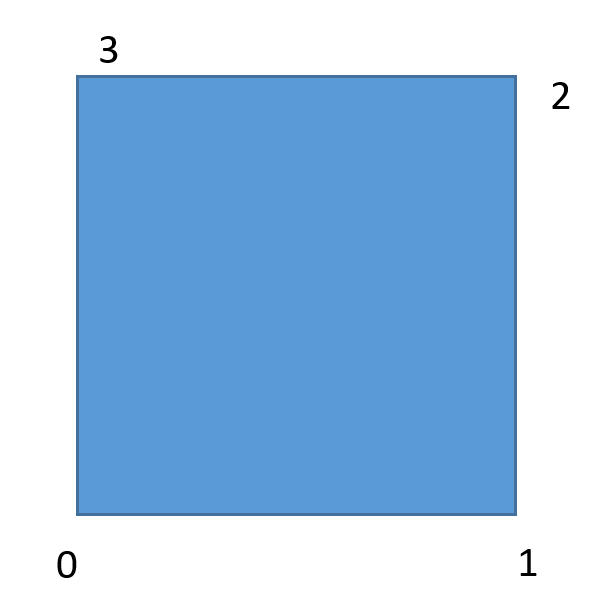
\includegraphics[width=0.3\textwidth]{element.png}
\caption[c]{Lokalna indeksacja węzłów elementu skończonego.}
\end{figure}

Macierz sztywności elementu $K$, dopóki nie zostaną na układ narzucone więzy unieruchamiające układ w przestrzeni jako ciało sztywne, jest osobliwa. Aby móc obliczyć przemieszczenia węzłów elementu pod działaniem określonych sił, nakładamy najpierw więzy. Załóżmy, że w naszym przypadku będą to więzy zamurowania lewego brzegu elementu, tzn. $x_0 = y_0 = x_3 = y_3 = 0$. W postaci macierzowej powyższe cztery równania są równoznaczne z zastąpieniem wierszy o indeksach 0, 1, 6 i 7 jedynkami na głównej diagonali macierzy i przypisaniu zer na tych indeksach w wektorze prawej strony. Po narzuceniu więzów macierz nie jest już osobliwa i można rozwiązać układ choćby procedurą Gaussa.

\subsection*{Zadania}
\begin{enumerate}
\item Napisz program, w którym zaalokujesz miejsce na macierz sztywności elementu, wektor przemieszczeń węzłowych oraz wektor prawych stron. Wykorzystaj tablicę {\tt fix[]} (opis poniżej) do narzucenia warunków brzegowych i rozwiąż zagadnienie procedurą Gaussa. Jako wymuszenie przyłóż siłę ciągnącą w dół prawy dolny węzeł.
\item Zmodyfikuj w programie obciążenie: przyłóż siłę skierowaną pionowo w dół do obu węzłów na prawej krawędzi. Rozwiąż zadanie. Następnie rozciągnij element. Sprawdź wpływ współczynnika Poissona na rozwiązanie. Pobaw się programem, aby zaznajomić się z zadawaniem obciążeń i ruchami poszczególnych stopni swobody.
\item Zmień sposób zamurowania na inny. Sprawdź, co się stanie z rozwiązaniem, gdy w ogóle nie narzucisz warunków brzegowych lub nie w pełni odbierzesz sztywne stopnie swobody układu.
\item Spróbuj stworzyć teraz belkę składającą się z dwóch elementów skończonych.
\end{enumerate}

\section{Wskazówki implementacyjne}
\begin{itemize}
\item Elementy w belce mają być indeksowane od 0 do $m_x*m_y-1$, poczynając od elementu w lewym dolnym rogu i indeksując je po kolei w prawo. Po dojściu do końca belki, zaczynamy od lewego brzegu analogicznie indeksować kolejnymi liczbami elementy w pasie położonym o jeden element wyżej niż dopiero co poindeksowany pas. W identyczny sposób indeksowane są węzły. Takiego indeksowania wymaga uproszczenie implementacji (brak transformacji geometrycznej macierzy sztywności) oraz prostota obecnej funkcji do rysowania całego układu.
\item {\tt mx} i {\tt my} oznaczają odpowiednio liczbę elementów w poziomie i w pionie w prostokątnej belce. Muszą to być zmienne globalne.
\item Funkcja do rysowania wymaga użycia globalnej tablicy {\tt int fix[2*(mx+1)*(my+1)]} o długości równej liczbie stopni swobody w siatce. Jeśli na danej pozycji w tablicy stoi zero, przyjmujemy, że ten stopień swobody ulega przemieszczeniom. Wpisanie na danym miejscu wartości 1, oznacza, że stopień swobody o tym indeksie jest odebrany (tak układ zostanie narysowany przez procedurę rysującą {\tt draw}). Oczywiście poprawność sformułowania matematycznego tak przyjętej konwencji i definicji tablicy {\tt fix[]} leży w pełni po stronie użytkownika. Takie zdefiniowanie tablicy {\tt fix} bardzo ułatwia implementację warunków brzegowych.
\item Początek głównego pliku z kodem programu powinien mieć następującą postać, aby uniknąć problemów z kolejnością definicji, nagłówkami i linkowaniem. Poniższy przykład pokazuje też sposób użycia biblioteki {\tt MesLib.h} w celu narysowania rozwiązanego układu.
\begin{verbatim}
#include <stdio.h>
#include "winbgi2.h"

const int mx = 1;
const int my = 1;

int fix[2*(mx+1)*(my+1)];

#include "MesLib.h"

int main()
{
   // Tu stworz caly program

   // Narysuj uklad
   graphics(700, 700);
   scale(0, 0.5*(my - mx - 3), mx + 3, 0.5*(my + mx + 3));
   title("X", "Y", "MES");
   draw(d, F);
   wait();
   
   // Zakoncz
   return 0;
}
\end{verbatim}
\end{itemize}

\section{Krótka dokumentacja biblioteki {\it MesLib.h}}
Biblioteka {\it MesLib.h} została stworzona na potrzeby laboratorium, aby uprościć i przyspieszyć implementację i zawiera szereg prostych i przydatnych funkcji oraz macierz sztywności i macierz masową pojedynczego elementu. Poniżej krótko opiszemy poszczególne funkcje:
\begin{itemize}
\item {\tt int P(int x, int y, int z)} - funkcja, która zwraca globalny indeks stopnia swobody przy założeniu, że {\it x} to jego indeks w kierunku x (liczony od 0 na lewej krawędzi), {\it y} to jego indeks w kierunku osi y (liczony od 0 na dolnej powierzchni belki), a {\it z} to 0 lub 1 zależnie od tego, czy interesuje nas stopień swobody w kierunku poziomym czy pionowym.
\item {\tt int Q(int x, int y)} - funkcja zwracająca globalny indeks elementu przy założeniu, że jest to element o indeksie {\it x} w kierunku poziomym i o indeksie {\it y} w kierunku pionowym.
\item {\tt int DOF(int elidx, int elidy, int locdofid)} - funkcja zwracająca globalny indeks stopnia swobody przy założeniu, że {\it elidx} oznacza indeks elementu w kierunku poziomym, {\it elidy} indeks elementu w kierunku pionowym, a {\it locdofid} to liczba od 0 do 7 oznaczająca lokalny indeks danego stopnia swobody. Lokalna indeksacja stopni swobody jest następująca: w węźle o indeksie 0 przesunięcia w kierunku poziomym i pionowym to odpowiednio $0-wy$ i $1-szy$ stopień swobody, w węźle o indeksie $1$ występują 2. i 3. stopień swobody itd.
\item Lokalna macierz sztywności jest zdefiniowana w dwuwymiarowej tablicy {\tt K[8][8]}. Przy składaniu macierzy sztywności powinna być w programie przemnożona przez czynnik {\tt Md} zawierający wpływ modułu Younga oraz współczynnika Poissona oraz przez grubość elementu.
\item Lokalna macierz masowa jest zdefiniowana w dwuwymiarowej tablicy {\tt M[8][8]}. Przy składaniu globalnej macierzy masowej powinna być w programie przemnożona przez czynnik {\tt Mm} zawierający wpływ gęstości materiału oraz dodatkowo należy ją przemnożyć przez grubość elementu.
\item {\tt void Gauss(int n, double **M, double *f, double *x)} - procedura eliminacji Gaussa rozwiązująca układ równań o macierzy zapisanej w dynamicznie zaalokowanej dwuwymiarowej tablicy {\tt M} o wymiarze {\tt n}, i wektorze prawej strony {\tt f}. Wynik zostanie wpisany do miejsc w pamięci wskazywanych przez wskaźnik {\tt *x}.
\item {\tt void draw(double *p, double *f)} - funkcja rysująca cały układ odkształconych elementów. {\tt p} to wektor przesunięć poszczególnych stopni swobody, a {\tt f} to wektor sił węzłowych w tych stopniach swobody. Ponadto funkcja wykorzystuje globalnie zadeklarowaną tablicę {\tt fix}, z której czerpie informację, które stopnie swobody układu są odebrane.
\end{itemize}

\end{document}